\chapter{MT history -- how has machine translation developed?}\label{sec:3}

    \objectives{
        You will learn...
        \begin{itemize}
            \item how MT developed in the last decades,  
            \item how the different MT systems generate their translation,
            \item how suitable the different MT architectures are with respect to post-editing. 
        \end{itemize}
        }

\vspace{\baselineskip}

You might get the impression that MT is a rather new invention because it became increasingly visible with the rise of statistical and especially neural MT engines. However, the first ideas about automating language and translation date back centuries. In order to understand which approaches are suitable for post-editing and under which conditions, it is important to learn something about the commonalities and differences of the MT architectures and how they developed over time. 

This section will shed light on the historical development of MT in \sectref{sec:3:1} and will introduce the basic MT approaches and discuss their suitability with respect to post-editing in \sectref{sec:3:2}.

\section{Historical development of MT}\label{sec:3:1}

The following table (\ref{long}) will show you the most important historical milestones starting from the 1930s with the first events that initiated the actual development of the first systems. The notion of automating translation processes is much older, however it was only theoretical then.

If you want to learn more about the historical development of MT, we recommend reading, for example, \citet{hutchins2000early}, \citet{hutchins2007machine}, and/or \citet{schwartz2018history}.

 \begin{longtable}[c]{ |>{\raggedright}p{2.8cm}||p{8.5cm}|  }
 \caption{History of MT.\label{long}}\\\hline
 \multicolumn{2}{| c |}{History of MT}\\\hline
 Event & Description\\\hline
 \endfirsthead
 
 \hline
 \multicolumn{2}{|c|}{History of MT}\\ \hline
 Event & Description\\ \hline
 \endhead
 
 \hline
 \endfoot
 
 \hline
 \multicolumn{2}{| c |}{Future}\\ \hline\hline
 \endlastfoot
 
 1933 - 
 
 First patents for ``Translating Machines" & The French-Armenian Georges Artsrouni and the Russian Petr Troyanskii independently proposed patents for ``translating machines" as early as 1933. Troyanskii proposed not only a method for an automatic bilingual dictionary on paper tape, but also a scheme for coding interlingual grammatical roles (based on Esperanto) and an outline of how analysis and synthesis might work. However, Troyanskii’s ideas were unknown to the community until the end of the 1950s.\\ \hline
 1949 - 
 
 Weaver Memorandum & A memorandum titled ``Translation" by Warren Weaver in July 1949 introduced the idea of MT to the general public. It is often considered the starting point of research on MT.\\ \hline
 1952 - 
 
 First MT conference & The first full-time researcher in MT was appointed at the Massachusetts Institute of Technology (MIT) in 1951, namely Yehoshua Bar-Hillel. He believed that fully-automatic, high-quality translation (FAHQT) could be possible. In 1952, the first conference on MT was held at MIT and covered topics such as pre-editing and post-editing, controlled language, domain restrictions, syntactic analysis as well as computer hardware, programming and funding.\\ \hline
 1954 - 
 
 Georgetown–IBM Experiment & During the Cold War, the first official MT projects were launched for the US military and also in the Soviet Union. Those projects focused on MT between Russian and English. They produced rather poor quality but were still popular for political and military reasons. Thus, most US research was for Russian-English translation, and most Soviet research was on English-Russian systems. The focus was on purely informative translation purposes without PE or any involvement of third-party translators or interpreters. 
 
 At Georgetown University, Leon Dostert collaborated with IBM on a project known as the Georgetown–IBM experiment which resulted in the first public demonstration of an MT system in January 1954. The project involved the fully automatic translation of more than sixty sentences from Russian into English. The experiment, which was conducted with well-chosen sentences, launched the first MT hype. This stimulated large-scale funding of MT research in the USA and inspired the initiation of MT projects elsewhere in the world, notably in the USSR.\\ \hline
 1961 - 
 
 Machine Translation Research in Texas & The Linguistic Research Center (LRC) at the University of Texas concentrated on basic syntactic research of English and German. Efforts were made to devise reversible grammars to achieve bidirectional translation within an essentially ``syntactic transfer" approach. This laid the foundations for the later successful development of the METAL system which started in 1979 in cooperation with Siemens AG.\\ \hline
 1966 - 
 
 ALPAC Report announces FAHQT impossible & In November 1966, the Automatic Language Processing Advisory Committee (ALPAC) issued a report to the Pentagon which brought the substantial funding of MT research in the United States to an end for about twenty years. The clear message of the ALPAC Report to the general public and the rest of the scientific community was that there is basically no hope for MT. The title of the report was ``Languages and machines: computers in translation and linguistics". Supposedly, it dealt not just with MT but also with computational linguistics. However, in practice, most funded NLP research was devoted to developing MT at the time.\\ \hline
 1968 - 
 
 The Beginnings of Systran & Engineering companies continued less visible research on MT. IBM developed the first commercial statistical machine translation system (SMT) Systran in 1968. Systran is one of the oldest MT companies and was founded by Peter Tome.\\ \hline
 1970-1978 - 
 
 Météo & In 1970, research began on a syntactic transfer system for English-French translation at Montreal. The TAUM project (Traduction Automatique de l'Université de Montréal) had two major achievements: the Q-system formalism, a computational metalanguage for manipulating linguistic strings and trees and the foundation of the Prolog programming language widely used in natural language processing; and secondly, the Météo system (1978) for translating English weather forecasts into French.\\ \hline
 1972-1986 - 
 
 SUSY & Researchers at Saarbrücken University developed SUSY (Saarbrücker Übersetzungssystem), a highly-modular multilingual transfer MT system.\\ \hline
 1976 - 
 
 EC and Systran & The European Commission first introduces Systran for in-house purposes.\\ \hline
 1978-1992 - 
 
 The EUROTRA project & The EUROTRA project was founded by the European Commission with the aim of developing a state-of-the-art MT system for the then seven, later nine, official languages of the European Community. In 1978, research on different MT projects began, e.g. research leading to the ARIANE system at Grenoble University (Russian-French-English-German), the LOGOS system (USA; now OpenLogos for German-English), and the GRADE system within the Mu project at Kyoto University (Japanese-English).\\ \hline
 1985 - 
 
 Prolog & In 1985, the Japanese government started the 5th Generation Project and developed the Prolog programming language for commercial MT which led to the development of LMT (Logic programming MT).\\ \hline
 1989 - 
 
 METAL System & Already in the 1970s, Siemens started working on a transfer approach for a machine translation system together with the LRC (Linguistic Research Centre) in Texas. Originally titled the Linguistics Research System (LRS), it was later renamed METAL (Mechanical Translation and Analysis of Languages) and finally became commercially available in 1989.\\ \hline
 1992 - 
 
 Automatic Evaluation of MT & The development of MT evaluation metrics started simultaneously with the development of statistical MT systems. Initial evaluations were carried out by human assessors according to FEMTI (Framework for the Evaluation of Machine Translation in ISLE). In 1992/1994, DARPA -- a research agency of the United States military -- investigated unedited output of MT systems, comparing automatic measures and human judgments of adequacy, fluency, informativeness.\\ \hline
 1993 - 
 
 Translation Memory Systems & The first commercial translation memory system, launched in the 1990s, was named TRADOS (TRAnslation and DOcumentation Software) and used aligned bilingual corpora. Trados was established in Stuttgart, Germany by Jochen Hummel and Iko Knyphausen in 1984. \\ \hline
 1997 - 
 
 First free online MT & After Systran started offering its service of online machine translations of entire webpages, the first free online machine translation was launched in December 1997 with Babel Fish on Alta Vista (later Yahoo) which was free for all Internet users but was discontinued in 2008.\\ \hline
 2000-2001 - 
 
 Crash of dotcom companies & After the crash of the dotcom companies in 2000, the number of MT software companies decreased to 10-20 active companies and universities that were working on MT. They made up only 1\% of revenue on the translation market despite the growing demand for MT applications. The still growing number of digitally available texts due to globalisation requires more translations with all sorts of language combinations even today.\\ \hline
 2001-2005 - 
 
 BLEU & In 2001, the BLEU score (Bilingual Evaluation Understudy) was developed which consists of statistical measures of similarity of SMT output and human (reference) translations. Other automatic evaluation scores include the NIST metrics by the National Institute of Standards and Technology and METEOR (Carnegie Mellon) in 2005.\\ \hline
 2002 - 
 
 Language Weaver & Language Weaver is the first company to commercialise a statistical approach to automatic language translation and natural language processing, which was founded by Kevin Knight and Daniel Marcu in 2002.\\ \hline
 2003-2004 - 
 
 Expansion of EU and growing demands & With the expansion of the EU, the number of official languages increased from 11 to 20 languages. At peak times, the European Union produced more than 1.4 million pages of text per month. Since then, about 380 language combinations are possible for translation at the EU, which can no longer only be covered by human translators.\\ \hline
 Since 2004 - 
 
 Open Source toolkits for MT & With the growing demand for language pairs numerous open source toolkits for MT systems appeared. Examples are: GIZA ++ (alignment tool for SMT); Moses (a platform for building SMT systems); Joshua (a decoder for syntax-based, hierarchical SMT); Apertium (a platform for building rule-based MT); META-SHARE (database for EU projects)\\ \hline
 2006 - 
 
 Google Translate SMT and Euromatrix & On 28 April 2006, Google Translate went online with a statistical MT system. The first system used transcripts from the UN and the European Parliament to gather enough training material. Further, the system used English as a transfer language. Later, Google expanded to further language pairs and applied a hybrid method. Around the same time, the Euromatrix project was founded with the aim of providing MT systems for all EU languages (over 500 language pairs), which involved a different research partner.\\ \hline
 2010 - 
 
 SDL Acquires Language Weaver & In July 2010, the leading language services company SDL acquired Language Weaver/ BeGlobal Statistical Machine Translation and the MT system became SDL Language Weaver.\\ \hline
 2016 - 
 
 Google introduces NMT & In 2016, Google Translate was one of the first to introduce neural machine translation (NMT). In November 2016, software engineer Harold Gilchrist, leader of the Google research team developing the Google Neural Machine Translation system (GNMT) to increase fluency and accuracy in Google Translate, announced the switch from SMT to GNMT.\\ \hline
 2016 - 
 
 SDL Adaptive MT & SDL introduces Adaptive MT for SDL Trados Studio 2017 - a self-learning machine translation engine.\\ \hline
 2017 - 
 
 DeepL is introduced & DeepL is another NMT system that was introduced by the online dictionary and corpora provider Linguee.\\ 
\end{longtable}




\section{MT architectures}\label{sec:3:2}

As you have seen above, different approaches have been developed to automatise the translation process. Here, we will discuss the pros and cons for rule-based, statistical and neural MT and their usability for PE workflows. 

\subsection{Rule-based machine translation (RBMT)}\label{sec:3:2:1}

Rule-based approaches were the catalyst for the development of MT. Generally, these systems attempt to define the individual characteristics of the source language and how these need to be converted into the target languages. \citet[31]{chesterman1997memes} mentions that he sees this early form of MT as “the Linguistic meme of translation theory”, because it assumes that languages can solely be expressed through rules, which, accordingly, must also be representable in algorithms. Different rule-based approaches had been developed over the years to generate MT:

 \begin{itemize}
    \item Direct MT: This type of MT is constructed specifically for one language pair and usually one translation direction. Essentially, the words of the source text are morphologically analysed and then looked up in a dictionary, which means that ideally all morphology rules are defined, so that the dictionary only has to contain the stems of the words. In the next steps, the words of the source language are replaced by the words in the target language and all morphological changes required by the target language are applied.
    \item Transfer-based MT: The transfer-based approach constructs a syntactic representation of the source text (often in a tree structure) that is free of ambiguities, etc. Next, this representation is generated for the target language with the help of a grammar that contains the bilingual transfer rules. The target text can be produced now. It is possible to use these systems in both language directions, but this is rarely done in practice, because the transfer rules often cannot be applied in both directions.
    \item Interlingua-based MT: For this approach, a so-called Interlingua needs to be created. This Interlingua represents meaning in an abstract form, which can theoretically be achieved by either a natural or an artificial language or a language-independent representation. The basic principle of this approach is that the source text is translated into the Interlingua and then the Interlingua into the target language. This approach is suitable for multilingual systems.
\end{itemize}

Please note that this is only a brief introduction to the main concepts of these approaches. For overviews on rule-based approaches see \citet{hutchins1992introduction} or \citet{wilks2008machine}. You can find a visualisation of the different rule-based approaches in \figref{fig:key:4:1}. This pyramid was introduced by \citet{vauquois1968survey} and shows the different steps that lie between source text and target text generation.

\begin{figure} 
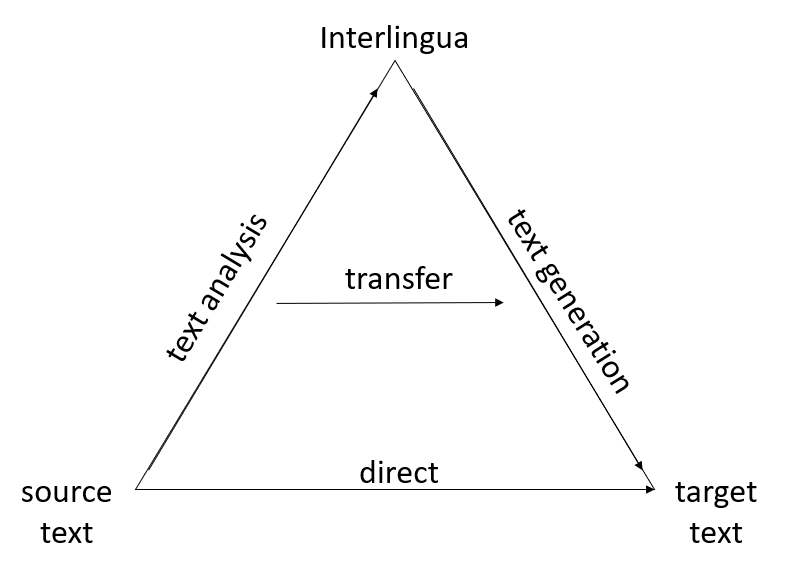
\includegraphics[height=0.4\textheight]{figures/Vaquoise triangle.PNG}
\caption{Vauquois pyramid \citep{vauquois1968survey}}
\label{fig:key:4:1}
\end{figure}


\largerpage[1.5]
Concerning PE, this approach seems especially suitable for the translation of texts adhering to a controlled language. Controlled languages are defined by a set of rules, which can theoretically be directly implemented into rule-based systems. The main disadvantage of these approaches is, however, that it takes a lot of effort to develop the systems, because the better and more comprehensive the intended system, the more rules have to be defined. If morphology, grammar, and syntax are only defined superficially, the source text might be generated incorrectly, which leads to (severe) mistakes in the target language. Further, the rules have to be defined from scratch for every language involved or sometimes even for every language direction, depending on the MT approach. 

Today, rule-based approaches are outdated and can usually only be found in hybrid systems or in very old, established systems. For example, the Pan American Health Organization (PAHO) still uses a rule-based system, because they already established their MT system in the 1980s and traditionally work with only three languages.\footnote{Find out more on the \href{https://www.paho.org/hq/index.php?option=com_content&view=article&id=14762:machine-translation-at-the-pan-american-health-organization&Itemid=1896&lang=en}{PAHO's webpage on their MT system PAHOMTS}, last accessed 27 April 2021.}\clearpage


More promising are data-based approaches, which render the human programming of linguistic rules for MT unnecessary. Data-based MT relies on mono- and multilingual corpus data. The following sections will give an overview of the most prominent data-based MT architectures: statistical machine translation (SMT) and neural machine translation (NMT).



\subsection{Statistical machine translation (SMT)}\label{sec:3:2:2}

SMT had been the state of the art for decades. The basic idea of this approach is to generate a translation from a parallel training corpus by calculating the most likely equivalent of a source word/phrase/sentence in the target language. Statistical translation models are generated and trained on corpus data. Both mono- and bilingual corpora are used to capture the typical linguistic structures of the languages involved – the monolingual corpora generate the target language model and the bilingual parallel corpora generate the translation model. In addition, SMT uses so-called n-grams – sequences of aligned words (usually n≤7) assigned with probabilities, which represent how likely the word sequences occur in the training corpus. Further, additional information can be extracted during the training phase, e.g. models of relative sentence length. The training of SMT systems can be realised relatively quickly if aligned parallel corpora are available. Training means in this context that the source text is analysed. Decoding, on the other hand, means in this context that the target text is generated. In between, there is the tuning phase, where the system tries to find the best values for the respective sentences or n-grams. Two models are commonly differentiated to calculate the most likely translation: the noisy channel model and the log-linear model. We do not want to go into detail here, please refer to \citet{hearne2011statistical} for further information.

In addition to the translation and language models, other features that contain linguistic information can be implemented to help calculate the most likely translation. These include a phrase table for each language direction, lexical translation probabilities, a model for phrase reordering, or a word or phrase penalty that controls the length of the target sentence. All these features help to calculate the most likely translation and select it among other translation candidates. Each feature obtains a value that represents its weight in the algorithm.

A final training task involves the evaluation of the system’s performance and the adaptation of the values that are given to the single features. One widely adopted technique to estimate the system is the so called MERT technique, which is short for Minimum Error Rate Training (see also \citealt{och2003minimum}). The MERT technique usually includes the BLEU metric. To keep it simple, this is an automatically calculated value that evaluates the quality of an MT system by comparing the translation output of the system to a reference translation.

An advantage of post-editing SMT texts is that the errors to be corrected are quite predictable. SMT systems always produce the same errors as long as they are not trained with new or extended training corpora. The code of the system is transparent and the calculation of translation probabilities straightforward. For a given language direction, typical errors can be identified, i.e. that the post-editor can systematically train error spotting and correction (\citealt{culo_influence_2014}, \citealt{nitzke2019problem}). 

Recent developments involving SMT have attempted to unite different approaches – usually rule-based and statistical – in hybrid systems so that the advantages of each approach can be combined. Systems with deep integration construct a whole new system that combines the advantages of the two approaches. Shallow integration systems, on the other hand, unite two or more existing systems into one new system.

\subsection{Neural machine translation (NMT)}\label{sec:3:2:3}

The latest approach to MT is the use of neural networks and can also be applied to parallel training corpora. NMT systems build large neural networks for translation, while statistical MT systems are composed of many small subcomponents. NMT systems use deep-learning approaches and learn automatically from the training data. 

At least three basic layers are involved in neural machine translation: the input layer, the output layer and at least one hidden layer in between. In the input layer, the source text is processed and in the output layer, the target text is created. The hidden layers are the processing steps. The model can work in a more fine-grained way and more complex tasks can be tackled when more hidden layers are included in a system. During training, mathematical representations and weights are assigned to the source and target segments in the training data. The training is comparably time-consuming as the system runs through the training data several times to adjust this structure. Further, no specific rules can be added manually, as the system develops the structure of the hidden layers automatically. Hence, only input and output layers are known, but the rest is more or less a blackbox (see \citealt{koehn2017neural} for detailed information), although tools and methods have been developed to interpret the decisions within a system (e.g. \citealt{vig2019bertviz})

Two approaches are common in neural machine translation: transformer and recurrent encoder-decoder models. In the encoding phase, the meaning of the source text is encoded into a vector with a fixed length. Transformer and recurrent systems differ in the way they encode the source text. In the decoder phase, the target segment is produced word for word. During the production, the system considers the surrounding words as context. One disadvantage of this system is that it has difficulties with long sentences. To overcome these problems, so called alignment models are implemented. These are often also called attention models. To improve the translation output, an additional layer is put between the input and the hidden layer. This additional layer embeds words, which means that the system is capable of considering context. This means that all content words are assigned to a representation. Words that are close content-wise are represented closely. Hence, similar words are clustered and are translated in similar manners. If you want to learn more on the architecture of NMT systems, read the comprehensible introduction by \citet{perez-ortiz_how_nodate}.

As the current NMT systems for interlingual translation currently outperform all other systems in many cases (\citealt{bentivogli2018neural}; \citealt{toral2017multifaceted}), not only redundant and highly standardised text types are in the focus of attention (as is the case in technical documentation, software localisation etc.), but also creative text types such as literary translation \citep{toral2018post} or subtitling \citep{tardel2020effort}. It might also be very interesting to test NMT for intralingual translation by translating Standard Language into Easy Language (as can be found in approaches to automatic text simplification, see \citealt{specia2010translating}). For example, it seems plausible that the neural networks might be able to represent the rules for translating standard German into Easy German during the training phase. For this purpose, a parallel corpus of standard German source texts and Easy German target texts will be necessary (e.g. \citealt{klaper2013building}). An NMT system which differentiates between different scales of complexity and difficulty (Easy Language -- Plain Language -- Standard Language -- Specialised Language) would revolutionise the whole area of accessible communication.

With respect to PE, one of the advantages of NMT is that the machine-trans\-lated output seems to be (much) better compared to other system architectures, at least when it comes to fluency. However, we can only get good results in the MT output if we have enough training material to feed the system. If we do not have enough training material, we get poor quality. This is often problematic for smaller languages and rare language combinations as they are often underrepresented and poor in resources. Further, as with all data-driven MT systems, the output can only be as good as the training data. Hence, if we train a system with poor quality translations, we get poor output. The same applies for domain specific translations. If the system is not well-trained on the specific domain, the output is poor as well. In total, the system is much more vulnerable to noisy data. Newest developments, however, allow the combination of NMT and the training of specific terminology, which tackles the domain problem (e.g. \citealt{michon2020integrating}). Another advantage is that NMT systems contain one compact system that does not have several components. However, training takes much longer than it takes for SMT and it also needs more computer processing capacities.

Finally, we want to point out that the generally better NMT output quality leaves us with the following paradox: the better the NMT translations are, the more difficult the error spotting is since the NMT output appears to be more fluent and less error-prone. This makes, on the one hand, the PE process even more demanding and leads to more cognitive effort for the post-editor. On the other hand, due to the absence of ``real" errors, the post-editors tend to correct more style errors, which in turn leads to over-editing (for details see \citealt{vardaro2019translation}). Hence, post-editors need a lot of training and awareness for the error types to be able to correct the texts efficiently.

\section*{Crossword puzzle -- chapter 3}

\begin{Puzzle}{15}{16}
|{}	|{}	|{}	|{}	|{}	|{}	|{}	|{}	|[6]W	|{}	|{}	|[8]S	|{} |{} |{} |.
|{}	|{}	|{}	|{}	|{}	|{}	|{}	|{}	|E	|{}	|{}	|T	|{} |{} |{} |.
|{}	|{}	|{}	|[3]R	|U	|S	|S	|I	|A	|N	|{}	|A	|{} |{} |{} |.
|{}	|{}	|{}	|{}	|{}	|{}	|{}	|{}	|T	|{}	|{}	|T	|{} |{} |{} |.
|[7]B	|A	|B	|E	|L	|F	|I	|S	|H	|{}	|{}	|I	|{} |{} |{} |.
|{}	|{}	|{}	|{}	|{}	|{}	|{}	|{}	|E	|{}	|{}	|S	|{} |{} |[9]I |.
|{}	|{}	|{}	|{}	|{}	|[2]G	|E	|O	|R	|G	|E	|T	|O |W |N |.
|{}	|{}	|{}	|{}	|{}	|{}	|{}	|{}	|F	|{}	|{}	|I	|{} |{} |T |.
|{}	|{}	|{}	|{}	|[10]N	|{}	|{}	|{}	|O	|{}	|{}	|S	|{} |{} |E |.
|{}	|{}	|{}	|[1]W	|E	|A	|V	|E	|R	|{}	|{}	|T	|{} |{} |R |.
|{}	|{}	|{}	|{}	|U	|{}	|{}	|{}	|E	|{}	|{}	|I	|{} |{} |L |.
|[5]S	|Y	|S	|T	|R	|A	|N	|{}	|C	|{}	|{}	|C	|{} |{} |I |.
|{}	|{}	|{}	|{}	|A	|{}	|{}	|{}	|[4]A	|L	|P	|A	|C |{} |N |.
|{}	|{}	|{}	|{}	|L	|{}	|{}	|{}	|S	|{}	|{}	|L	|{} |{} |G |.
|{}	|{}	|{}	|{}	|{}	|{}	|{}	|{}	|T	|{}	|{}	|{}	|{} |{} |U |.
|{}	|{}	|{}	|{}	|{}	|{}	|{}	|{}	|S	|{}	|{}	|{}	|{} |{} |A |.
\end{Puzzle}

\begin{PuzzleClues}{\textbf{Across}}
\Clue{1}{WEAVER}{Who wrote the memorandum titled ``Translation" published in 1949?}
\Clue{2}{GEORGETOWN}{Which university hosted the first public demonstration of an MT system in January 1954?}
\Clue{3}{RUSSIAN}{Which languages were involved in the first public demonstration of an MT system in January 1954? English and ...}
\Clue{4}{ALPAC}{What was the name (abbreviation) of the report that ended funding of MT research in the United States for about twenty years?}
\Clue{5}{SYSTRAN}{What is the name of one of the oldest MT companies that was founded by Peter Tome?}
\Clue{7}{BABELFISH}{What was the name of the first free online machine translation that was launched in December 1997?}
\end{PuzzleClues}

\begin{PuzzleClues}{\textbf{Down}}
\Clue{6}{WEATHERFORECASTS}{What was translated by the Météo system?}
\Clue{8}{STATISTICAL}{With what kind of approach did Google launch their first online MT system?}
\Clue{9}{INTERLINGUA}{What is the name of a language that represents meaning in an abstract form?}
\Clue{10}{NEURAL}{What is the state-of-the-art MT approach? ... MT}
\end{PuzzleClues}
